\documentclass{article}
\usepackage{sc2025_paper_template}
\usepackage{times}
\usepackage{ifpdf}
\usepackage{soul}
\usepackage{subcaption}
\usepackage[english]{babel}

\def\papertitle{SCKinect \\ 
\large A SuperCollider plugin for the Kinect}
\def\firstauthor{Evan Murray}
\def\secondauthor{Henrik von Coler}

% pdf-tex settings: detect automatically if run by latex or pdflatex
\newif\ifpdf
\ifx\pdfoutput\relax
\else
   \ifcase\pdfoutput
      \pdffalse
   \else
      \pdftrue
  \fi
\fi

\ifpdf % compiling with pdflatex
  \usepackage[pdftex,
    pdftitle={\papertitle},
    pdfauthor={\firstauthor, \secondauthor},
    bookmarksnumbered, % use section numbers with bookmarks
    pdfstartview=XYZ % start with zoom=100% instead of full screen; 
                     % especially useful if working with a big screen :-)
   ]{hyperref}

  \usepackage[pdftex]{graphicx}
  % declare the path(s) where your graphic files are and their extensions so 
  %you won't have to specify these with every instance of \includegraphics
  \graphicspath{{./figures/}}
  \DeclareGraphicsExtensions{.pdf,.jpeg,.png}

  \usepackage[figure,table]{hypcap}

\else % compiling with latex
  \usepackage[dvips,
    bookmarksnumbered, % use section numbers with bookmarks
    pdfstartview=XYZ % start with zoom=100% instead of full screen
  ]{hyperref}  % hyperrefs are active in the pdf file after conversion

  \usepackage[dvips]{epsfig,graphicx}
  % declare the path(s) where your graphic files are and their extensions so 
  %you won't have to specify these with every instance of \includegraphics
  \graphicspath{{./figures/}}
  \DeclareGraphicsExtensions{.eps}

  \usepackage[figure,table]{hypcap}
\fi

%setup the hyperref package - make the links black without a surrounding frame
\hypersetup{
    colorlinks,
    citecolor=black,
    filecolor=black,
    linkcolor=black,
    urlcolor=black
}

\title{\papertitle}

\twoauthors
{0.5in}
{\firstauthor} {Georgia Institute of Technology \\
    {\tt \href{mailto:evan@auraaudio.io}{evan@auraaudio.io}}}
{\secondauthor} {Georgia Institute of Technology \\
    {\tt \href{mailto:hvc@gatech.edu}{hvc@gatech.edu}}}

\usepackage{cleveref}
\begin{document}

\capstartfalse
\maketitle
\capstarttrue

\begin{abstract}
SCKinect is a SuperCollider plugin that allows users to interact with a Kinect sensor. Its core implementation contains a unit generator called 'Kinect', designed to output motion-tracking data to control buses. The plugin also includes commands, facilitating interaction with Kinect devices through the interpreter. The interpreted nature of SuperCollider and the server-language duality allow multimedia enthusiasts to efficiently communicate with technical rendering systems. This is perfect for live performances and interactive installations. With the addition of this plugin, performers can interact with the Kinect directly in SuperCollider with low latency. This paper will cover the implementation of the plugin and its potential applications.
\end{abstract}

\section{Background}\label{sec:background}
According to~\cite{noauthor_fastest-selling_nodate}, the record for the fastest-selling gaming peripheral was set by the Kinect on January 3rd, 2011. The device sold on average 133,333 units per day in the first 60 days of its launch. Featuring a custom System on Chip, originally developed by PrimeSense, this device was designed to be good at detecting people and their surrounding environment~\cite{boehm_natural_2012}. In fact, it almost did this too well. Naturally, users became skeptical of the sensors built into the device and their privacy implications, as described in~\cite{de_guzman_security_2020}. This, in combination with numerous other factors, led to the eventual decline of the Kinect as a consumer product over the next decade. According to~\cite{peters_microsoft_2023}, the last Kinect product (Kinect Azure) was discontinued in October 2023, marking over a decade-long life-cycle for this product.
\section{Motivation}\label{sec:motivation}
If the Kinect was already discontinued and no longer being supported by its official creator, a valid question to ask is: why should one continue using it? Even better: how might one use it with SuperCollider? Musicians, whether they realize it or not, inherently control numerous parameters on their instrument--leading to a unique musical expression. To match the sound of a babbling crowd at a restaurant, a trombone player might mask their melody with a plunger mute to get that classic "wah wah" sound. In electronic music, a synthesizer performer or DJ might turn the knobs on their device which control the cutoff frequency of a highpass filter. This is typically done to prepare the crowd for a major transition in the song. In interactive programming languages, such as SuperCollider, performers don't have these knobs or tactile interfaces which physical instruments might offer. However, they can be implemented by connecting a joy stick or mouse as a Human Interaction Device. This will allow the performer to have some tactile input which they can use to control a particular parameter in their program, influencing the sound or visual output which is created.
\section{Natural User Interfaces}\label{sec:natural_user_interfaces}
There are a class of user interfaces which are encompassed under the term, Natural User Interfaces. These types of interfaces, according to~\cite{norman_natural_2010}, bypass conventional ones (such as the mechanical mouse and keyboard).~\cite{jacob_reality-based_2008} further classifies these as Reality-Based Interfaces (RBI). Something compelling about these is their aim to intuit real-world interactions. One of the themes mentioned in~\cite{jacob_reality-based_2008} related to RBI is body awareness and skills, which describes how "people have an awareness of their own physical bodies and posses skills for controlling and coordinating their bodies." This is what neuroscientists would call "proprioception." Virtual Reality devices take this into account with their head-mounted displays. Instead of interacting by keyboard or mouse, the user can tilt their head in different directions as they would in the real world.
\section{Kinect Interface}\label{sec:sckinect}
Using the Kinect and a couple of open-source helper tools, tracking a user's full body motion with high precision is possible. This is an alternative to using a VR headset with a tracker (required for full-body tracking in VR). Furthermore, the Kinect is much cheaper than the combined price of a VR headset and a tracker. Based on what was discussed previously in \ref{sec:motivation}, this motion tracking tool can be used similar to a Human Interaction Device in SuperCollider, allowing the user to map body movements to control busses. A caveat to this, discussed in \ref{subsec:nvidia_gtx_1080_gpu}, is depending on the implementation--some sophisticated hardware may be required to perform with low latency. This typically requires a Graphical Processing Unit (GPU) to help the Central Processing Unit (CPU) with absurd amounts of data. The data comes from a pose estimation model which relies on machine learning algorithms. It's worth noting over the last decade, GPU's and CPU's have become smaller and more affordable--making their use a bit more practical to the average consumer. In addition, there are plenty of algorithms which don't rely on machine learning, such as the application of Dijkstra’s algorithm demonstrated in~\cite{fossati_data-driven_2013}. These algorithms can perform low-latency human pose estimation on the CPU. A future goal of SCKinect is to incorporate algorithms similar to these for non-GPU users. However, for the sake of simplicity--the discussion below will focus on all the hardware and software components used in constructing the GPU-based machine learning approach.
\section{Hardware Components}\label{sec:hardware_components}
The hardware components which made this project possible are described below. It's important to note the Kinect v2 needs a separate USB adapter for connecting to the computer, which costs around 20-40 US dollars. The Kinect v1 has an adapter which is sold for around half the price.
\subsection{AMD Ryzen 5 3600 CPU}\label{subsec:amd_ryzen_5_3600_cpu}
This CPU shown in Figure \ref{subfig:cpu} was chosen for this project because it has a nice performance which doesn't cause the GPU to bottleneck. The Ryzen 5 3600 sells for about 40-80 US dollars with a base clock speed of 3.6 GHz and 6 cores with 12 threads.
\subsection{NVIDIA GTX 1080 GPU}\label{subsec:nvidia_gtx_1080_gpu}
The GPU shown in Figure \ref{subfig:gpu} was chosen for its compatibility with the pose estimation model. This is probably the most expensive hardware component of this project, selling for about 150-200 US dollars for a refurbished device. However, as noted previously--further options are being explored for CPU-only pose estimation. Additionally, NVIDIA's competitor--AMD--sells similar GPU's for about half of the price. Thus, it may be worth further investigation to explore adding support for other GPU brands as well.
\subsection{Kinect}\label{subsec:kinect}
The Kinect v2, pictured in Figure \ref{subfig:kinect}, is currently one of the cheapest Red Green Blue Depth (RGB-D) cameras on the market, selling pre-owned for about 50-100 US dollars. The Kinect v1 sells at about half the price with slightly lower specifications. At this time, SCKinect currently only supports 2D tracking. Thus, one technically doesn't need a Kinect and could use a camera instead. However, incorporating depth data into the existing pose estimation model is currently being explored. The Kinect v2 features a 1920x1080 resolution color camera, as well as a 512x424 resolution depth camera. The depth is based on the Time of Flight (ToF) sensors which put out infared light. It also has a 70x60 degree field of view and a 4-channel microphone array, which records audio at 48 kHz. There are also other methods of doing 3-dimensional (3D) pose tracking besides using an RGB-D camera (i.e. stereoscopic cameras). However, using an RGB-D camera as opposed to a stereoscopic setup may yield a higher resolution indoors, while stereoscopic cameras are better for use outdoors (since the sun's infared rays will overpower the Kinect's infared). One may also consider using multiple RGB-D and stereoscopic cameras for improved flexibility.

\begin{figure}[t!]
\centering
\begin{subfigure}[t]{0.32\columnwidth}
    \centering
    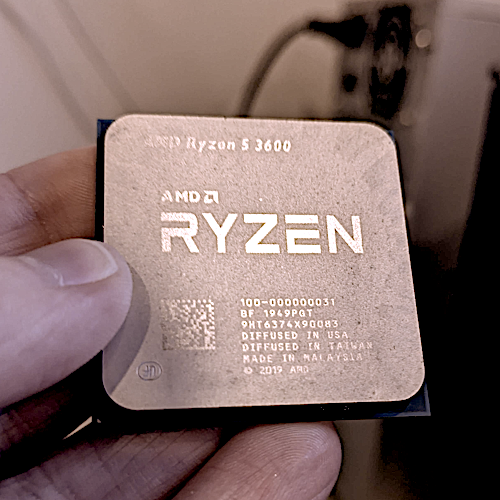
\includegraphics[width=1\textwidth]{CPU.png}
    \caption{Ryzen 5 3600\label{subfig:cpu}}
\end{subfigure}
\begin{subfigure}[t]{0.32\columnwidth}
    \centering
    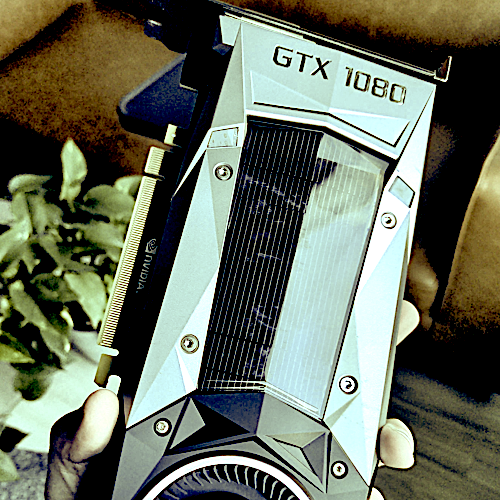
\includegraphics[width=1\textwidth]{GPU.png}
    \caption{GTX 1080\label{subfig:gpu}}
\end{subfigure}
\begin{subfigure}[t]{0.32\columnwidth}
    \centering
    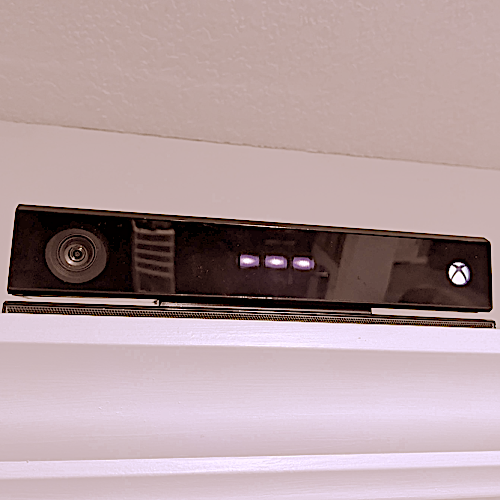
\includegraphics[width=1\textwidth]{Kinect.png}
    \caption{Kinect v2\label{subfig:kinect}}
\end{subfigure}
\caption{A picture of the three essential hardware components for the project.\label{fig:hardware}}
\end{figure}

\section{Software Components}\label{sec:components}
\subsection{Libfreenect2}\label{subsec:libfreenect2}
Libfreenect2, as shown in~\cite{lingzhu_xiang_libfreenect2_2016}, is a library created by open-source developers for retrieving data from the Kinect. This data does not include pose estimations, but it includes all of the functions needed for interacting with the Kinect (i.e. opening, closing, and starting a stream of data).
\subsection{OpenPose}\label{subsec:openpose}
OpenPose is the library responsible for returning the pose estimation data, pictured in Figure \ref{fig:pose}. It was developed by the Perceptual Computing Lab at Carnegie Mellon University and uses Convolutional Neural Networks to do marker-less motion tracking. This tracking data includes 24 different joints on the human body. See~\cite{8765346, simon2017hand, cao2017realtime, wei2016cpm} for more information.
\section{Implementation}\label{sec:implementation}
SCKinect is implemented as a SuperCollider 3 plugin, featuring server commands for interacting with the components discussed in \ref{subsec:libfreenect2} and \ref{subsec:openpose} respectively. The full source code is available on \href{https://github.com/L42i/SCKinect}{GitHub}\footnote{\href{https://github.com/L42i/SCKinect}{https://github.com/L42i/SCKinect}\label{footnote:sckinect_github}}. Currently, the plug-in works best if installed on Ubuntu 20.04. However, future releases will include support for both macOS and Windows--with or without a GPU.

\begin{figure}[htbp]
\centering
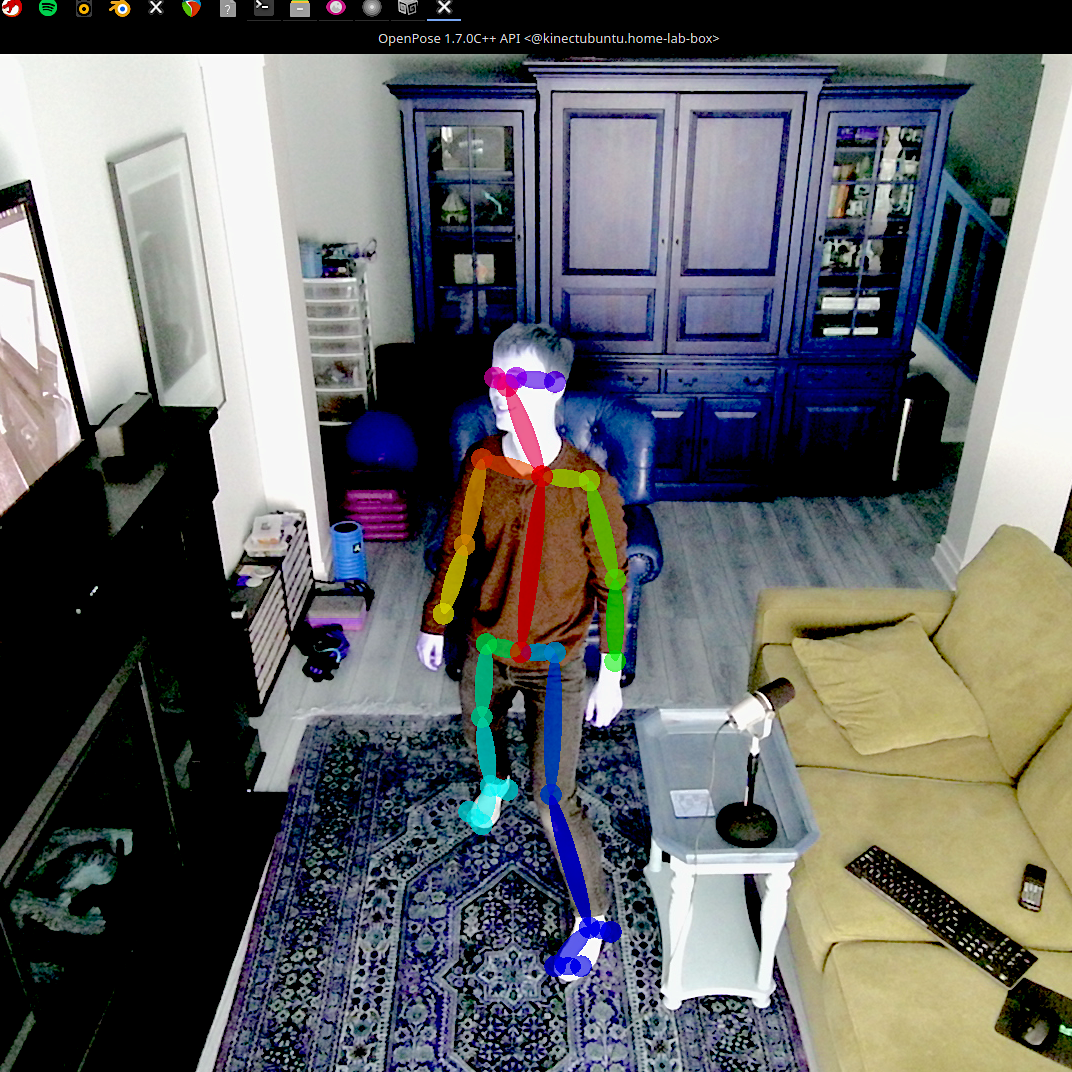
\includegraphics[width=0.9\columnwidth]{Pose.png}
\caption{The window displayed in SCKinect which shows the 24 joints being tracked on the human body real-time. \label{fig:pose}}
\end{figure}

\section{Commands}\label{sec:commands}
Commands allow SuperCollider to pass parameters from a SuperCollider class to the plugin, allowing one to configure the Kinect and OpenPose directly from SuperCollider. The currently implemented commands are explained below. They should also be run in the order they are shown when using SuperCollider.
\subsection{\texttt{Kinect.findAvailable}}\label{subsec:kinect_find_available}
This is designed similar to the \texttt{HID.findAvailable} command in SuperCollider. It queries all of the Kinect devices connected to the computer and posts their serial numbers to the post window, as shown below:\\
\texttt{\\
-> Kinect\\
{[Info]} {[Freenect2Impl]} enumerating \\ devices...\\
{[Info]} {[Freenect2Impl]} 12 usb devices \\ connected\\
{[Info]} {[Freenect2Impl]} found valid \\ Kinect v2 @4:4 with serial \\ 008953333347\\
{[Info]} {[Freenect2Impl]} found valid \\ Kinect v2 @4:2 with serial \\ 065915234247\\
{[Info]} {[Freenect2Impl]} found 2 \\ devices
}

\subsection{\texttt{Kinect.setPipeline}}\label{subsec:kinect_set_pipeline}
This command determines the device responsible for passing the data from the Kinect to OpenPose. The possible pipelines are Dump, CPU, OpenGL, CUDA, and CUDAKDE. For example, if one wanted to set the pipeline to use CUDA (assuming they have an NVIDIA GPU and the CUDA toolkit installed), they could run the command:\\
\\
\texttt{Kinect.setPipeline("CUDA")}
\subsection{\texttt{Kinect.openDevice}}\label{subsec:kinect_open_device}
\texttt{Kinect.openDevice} opens the device with the given serial number. For example, the second device shown in the output of running the command in \ref{subsec:kinect_find_available} is opened by running:\\
\\
\texttt{Kinect.openDevice("065915234247")}
\subsection{\texttt{Kinect.start}}\label{subsec:kinect_start}
This command will tell \texttt{libfreenect2} to start preparing the Kinect for processing frames.
\subsection{\texttt{Kinect.configureTracking}}\label{subsec:kinect_configure_tracking}
This command configures the OpenPose model with specific settings. There are a lot of parameters which will be documented in \cref{footnote:sckinect_github} \Cpageref{footnote:sckinect_github}. However, the most important one to understand is the path to the model folder, \texttt{"/home/emurray49/openpose/models"}. As opposed to the folder shown below, an existing path should be passed to the function instead. More instructions are available on \href{https://emurray2.github.io/spatial-auditory-feedback/kinect/\#openpose}{GitHub Pages}\footnote{\href{https://emurray2.github.io/spatial-auditory-feedback/kinect/\#openpose}{https://emurray2.github.io/spatial-auditory-feedback}\label{footnote:spatial_auditory_feedback_github_pages}}. Here is what the full command might look like:\\\texttt{\\
    Kinect.configureTracking\\
    (\\
    3, 1,\\
    "/home/emurray49/openpose/models",\\
    1, 0, 1, 0.25,\\
    0, "-1x-1", "-1x256",\\
    1, "BODY\_25", 0.5,\\
    0.5, 0, 0.05, -1, 0.0\\
    )
}

\subsection{\texttt{Kinect.startTracking}}\label{subsec:kinect_start_tracking}
If the previous commands run successfully, one may start the motion tracking by running this command. Upon running this command, the pose tracking window will be displayed, as shown in Figure \ref{fig:pose}.
\subsection{\texttt{Kinect.hideDisplay}}\label{subsec:kinect_hide_display}
If one wishes to hide this display of the pose tracking, they may disable it by running the above command.
\subsection{\texttt{Kinect.showDisplay}}\label{subsec:kinect_show_display}
To re-enable the pose tracking display, one may run this command after it has been disabled.
\subsection{\texttt{Kinect.stopTracking}}\label{subsec:kinect_stop_tracking}
This will stop the motion tracking and hide the display window if shown.
\subsection{\texttt{Kinect.stop}}\label{subsec:kinect_stop}
This command will stop the Kinect frames.
\subsection{\texttt{Kinect.closeDevice}}\label{subsec:kinect_close_device}
\texttt{Kinect.closeDevice} closes the device with the given serial number. For example, the device shown in the output of running the command in \ref{subsec:kinect_find_available} is closed by running:\\
\\
\texttt{Kinect.closeDevice("065915234247")}
\section{Mapping}
The \texttt{Kinect} UGen included in the SCKinect plugin includes a \texttt{.kr} method for mapping a specific joint to a control bus. Consider the following example of creating two control busses for a synthesizer:\\
\texttt{\\
    $\sim$amplitudeBus = Bus.control(s, 1);\\
	$\sim$frequencyBus = Bus.control(s, 1);\\
}

The first bus could be used to control the amplitude and the second bus could be used to control the frequency. The next goal is to map joints on the human body to these parameters. How about mapping the y position of the right wrist to the amplitude and the x position of the left wrist to the frequency? Here is what that might look like:\\
\texttt{\\
    var a = $\sim$kinectAmplitudeBus.index;\\
    var b = $\sim$kinectFrequencyBus.index;\\
    var e = "RWrist";\\
    var f = "LWrist";\\
    var c = Kinect.kr(0, 0.5, e, "Y");\\
    var d = Kinect.kr(20, 10000, f, "X");\\
    \{Out.kr(a, c)\}.play;\\
	\{Out.kr(b, d)\}.play;\\
}

This creates two Kinect Unit Generators ("RWrist" and "LWrist") and maps their "Y" and "X" positions, given by the \texttt{.kr} outputs, to the amplitude and frequency busses respectively. Notice how the desired bounds of each control input are also specified: amplitude being \texttt{0-0.5} and frequency being \texttt{20-10000} Hertz. A full example of this code is available in the \texttt{examples} folder of \cref{footnote:sckinect_github} \Cpageref{footnote:sckinect_github}. The full list of joint names which are possible are found in the \href{https://cmu-perceptual-computing-lab.github.io/openpose/web/html/doc/md\_doc\_02\_output.html\#autotoc\_md41}{OpenPose documentation}\footnote{\href{https://cmu-perceptual-computing-lab.github.io/openpose/web/html/doc/md\_doc\_02\_output.html\#autotoc\_md41}{https://cmu-perceptual-computing-lab.github.io/openpose/}\label{footnote:openpose_documentation}}.

\section{Conclusion}
In conclusion, SCKinect provides a direct interface to the Kinect in SuperCollider. This allows people to turn their whole body into an immersive controller. Future goals of this plugin are to support other GPU brands and non-GPU based algorithms for performing pose estimation. In addition, a workflow for outputting a "Z" coordinate for each joint, along with the "X" and "Y" coordinates, will be developed. Contributions and feedback are welcome at the repository listed in \cref{footnote:sckinect_github} on \Cpageref{footnote:sckinect_github}.

\bibliography{sckinect}

\end{document}
